\chapter{Python's Object Oriented Programming}\label{introduction-to-python---lesson-2}

In this chapter the main characteristics that makes $\tt{python}$ an \textit{object oriented programming} language will be reviewed.
Before going to OOP the concept of function and variable scope will be outlined.

\section{Functions}\label{functions}

A function is a block of organized, reusable code that is used to perform a single action. Functions provide better modularity for your application and high degree of code reusing.
To define a function the keyword \texttt{def} is used, followed by the name of the function and by the required parameters in parenthesis.

\begin{Verbatim}[commandchars=\\\{\}]
\PY{c+c1}{\PYZsh{} sum up all the integers between 1 and n }
\PY{k}{def} \PY{n+nf}{my\PYZus{}function}\PY{p}{(}\PY{n}{n}\PY{p}{)}\PY{p}{:} \PY{c+c1}{\PYZsh{} this function take one input only (n)}
    \PY{n}{x} \PY{o}{=} \PY{l+m+mi}{0}
    \PY{k}{for} \PY{n}{i} \PY{o+ow}{in} \PY{n+nb}{range}\PY{p}{(}\PY{l+m+mi}{1}\PY{p}{,} \PY{n}{n}\PY{o}{+}\PY{l+m+mi}{1}\PY{p}{)}\PY{p}{:}
        \PY{n}{x} \PY{o}{+}\PY{o}{=} \PY{n}{i}
    \PY{k}{return} \PY{n}{x} \PY{c+c1}{\PYZsh{} the function returns a number}

\PY{n}{my\PYZus{}function}\PY{p}{(}\PY{l+m+mi}{5}\PY{p}{)} \PY{c+c1}{\PYZsh{} 5 + 4 + 3 + 2 + 1}
\end{Verbatim}

Functions can return any kind of objects (numbers, strings, lists, complex objects\ldots{}) but it is not mandatory to have a return value, so you can have functions \textbf{without} a \texttt{return} statement (e.g. a function that simply take a string as input and print it to screen with a particular format).
In addition the syntax of the \texttt{return} is different from other languages like \texttt{Visual\ Basic}, the returned object doesn't have to have the same name as the function. Indeed above the variable $\tt{x}$ is returned and not the variable $\tt{my_function}$.

\begin{Shaded}
\begin{Highlighting}[]
\KeywordTok{def}\NormalTok{ printing(mystring):}
    \BuiltInTok{print}\NormalTok{((myString)}\BuiltInTok{.upper())}
\end{Highlighting}
\end{Shaded}

Functions can call other functions (once a function has been defined it can be accessed from everyone withing the same file or notebook): here $\tt{my_function_2}$ calls $\tt{my_function}$

\begin{Verbatim}[commandchars=\\\{\}]
\PY{k}{def} \PY{n+nf}{my\PYZus{}function\PYZus{}2}\PY{p}{(}\PY{n}{n}\PY{p}{,} \PY{n}{x}\PY{p}{)}\PY{p}{:} 
   \PY{k}{return} \PY{l+s+s2}{\PYZdq{}}\PY{l+s+s2}{The result is : }\PY{l+s+si}{\PYZob{}\PYZcb{}}\PY{l+s+s2}{\PYZdq{}}\PY{o}{.}\PY{n}{format}\PY{p}{(}\PY{n+nb}{str}\PY{p}{(}\PY{n}{my\PYZus{}function}\PY{p}{(}\PY{n}{n}\PY{p}{)}\PY{o}{*}\PY{n}{x}\PY{p}{)}\PY{p}{)}
   \PY{c+c1}{\PYZsh{} returns x * result of my\PYZus{}function(n)}
   \PY{c+c1}{\PYZsh{} so function of function}

\PY{n}{my\PYZus{}function\PYZus{}2}\PY{p}{(}\PY{l+m+mi}{5}\PY{p}{,} \PY{l+m+mi}{10}\PY{p}{)}
\end{Verbatim}

Functions can also call themselves too (i.e \emph{recursion}). In the next example we will see a function that computes the factorial exploiting the following relationship:

\[
\begin{cases}
    n! = n \times (n-1)! & \;\; (\forall n \gt 1) \\
    n! = 1 & \;\; (\forall n \le 1)
\end{cases}
\]

\begin{Verbatim}[commandchars=\\\{\}]
\PY{k}{def} \PY{n+nf}{factorial}\PY{p}{(}\PY{n}{n}\PY{p}{)}\PY{p}{:}
   \PY{k}{if} \PY{n}{n} \PY{o}{\PYZlt{}}\PY{o}{=} \PY{l+m+mi}{1}\PY{p}{:}
      \PY{k}{return} \PY{l+m+mi}{1}
   \PY{k}{else}\PY{p}{:}
      \PY{k}{return} \PY{n}{n} \PY{o}{*} \PY{n}{factorial}\PY{p}{(}\PY{n}{n}\PY{o}{\PYZhy{}}\PY{l+m+mi}{1}\PY{p}{)}

\PY{n}{factorial}\PY{p}{(}\PY{l+m+mi}{10}\PY{p}{)}
\end{Verbatim}

In this example the function $\tt{factorial}$ is initially called with the input corresponding to the factorial we want to compute, it then call itself each time with $\tt{n-1}$, multypling together all the results.

The previous example is quite simple but recursion can be tricky sometimes so apply it with caution. 

Functions input parameters also accept default values, which means that a function that works with some input values can be called with less parameters provided their default values have been specified.

In the following example the function $\tt{powers}$ takes three inputs: a list of numbers, an exponent ($\tt{n}$) and a constant ($\tt{c}$). The code loops through the provided list of numbers and process them according to the formula $item^{n} + c$, it puts the results in a new list which will be finally returned.

\begin{tcolorbox}[breakable, size=fbox, boxrule=1pt, pad at break*=1mm,colback=cellbackground, colframe=cellborder]
\begin{Verbatim}[commandchars=\\\{\}]
\PY{k}{def} \PY{n+nf}{powers}\PY{p}{(}\PY{n}{l}\PY{p}{,} \PY{n}{n}\PY{o}{=}\PY{l+m+mi}{2}\PY{p}{,} \PY{n}{c}\PY{o}{=}\PY{l+m+mi}{0}\PY{p}{)}\PY{p}{:}
    \PY{k}{return} \PY{p}{[}\PY{n}{item}\PY{o}{*}\PY{o}{*}\PY{n}{n}\PY{o}{+}\PY{n}{c} \PY{k}{for} \PY{n}{item} \PY{o+ow}{in} \PY{n}{l}\PY{p}{]}

\PY{n+nb}{print} \PY{p}{(}\PY{n}{powers}\PY{p}{(}\PY{p}{[}\PY{l+m+mi}{5}\PY{p}{,} \PY{l+m+mi}{11}\PY{p}{,} \PY{l+m+mi}{6}\PY{p}{]}\PY{p}{,} \PY{l+m+mi}{3}\PY{p}{,} \PY{l+m+mi}{4}\PY{p}{)}\PY{p}{)}
\PY{n+nb}{print} \PY{p}{(}\PY{n}{powers}\PY{p}{(}\PY{p}{[}\PY{l+m+mi}{5}\PY{p}{,} \PY{l+m+mi}{11}\PY{p}{,} \PY{l+m+mi}{6}\PY{p}{]}\PY{p}{)}\PY{p}{)}

[129, 1335, 220]
[25, 121, 36]
\end{Verbatim}
\end{tcolorbox}
    
As you can see in the example the function is called twice with two different set of parameters: in the first case we pass to it the list of numbers, the exponent and the costant, in the second only just the same list of numbers.
In the latter case, being defined the default values for $\tt{n}$ and $\tt{c}$, the function works as well, fewer inputs are provided and the missing ones will be replaced by their defaults. 

When calling a function paramenters can be passed also by name for clarity, in this case of course the order doesn't matter. Compare the two results below:

\begin{tcolorbox}[breakable, size=fbox, boxrule=1pt, pad at break*=1mm,colback=cellbackground, colframe=cellborder]
\begin{Verbatim}[commandchars=\\\{\}]
\PY{k}{def} \PY{n+nf}{func}\PY{p}{(}\PY{n}{a}\PY{p}{,} \PY{n}{b}\PY{p}{,} \PY{n}{c}\PY{p}{)}\PY{p}{:}
    \PY{k}{return} \PY{n}{a} \PY{o}{+} \PY{n}{b} \PY{o}{*} \PY{n}{c}

\PY{n+nb}{print} \PY{p}{(}\PY{n}{func}\PY{p}{(}\PY{n}{c}\PY{o}{=}\PY{l+m+mi}{4}\PY{p}{,} \PY{n}{b}\PY{o}{=}\PY{l+m+mi}{2}\PY{p}{,} \PY{n}{a}\PY{o}{=}\PY{l+m+mi}{1}\PY{p}{)}\PY{p}{)}
\PY{n+nb}{print} \PY{p}{(}\PY{n}{func}\PY{p}{(}\PY{l+m+mi}{4}\PY{p}{,} \PY{l+m+mi}{2}\PY{p}{,} \PY{l+m+mi}{1}\PY{p}{)}\PY{p}{)}

9
6
\end{Verbatim}
\end{tcolorbox}

In the first case the function is called by name, in the second case the parameter are implicitly assinged according to thier position.

Another nice feature of $\tt{pyhton}$ functions is that we can associate an help message to them so that we can easily check what a function is for by simply asking $\tt{help(functioName)}$:

\begin{tcolorbox}[breakable, size=fbox, boxrule=1pt, pad at break*=1mm,colback=cellbackground, colframe=cellborder]
\begin{Verbatim}[commandchars=\\\{\}]
\PY{k}{def} \PY{n+nf}{powers}\PY{p}{(}\PY{n}{l}\PY{p}{,} \PY{n}{n}\PY{o}{=}\PY{l+m+mi}{2}\PY{p}{,} \PY{n}{c}\PY{o}{=}\PY{l+m+mi}{0}\PY{p}{)}\PY{p}{:}
    \PY{l+s+sd}{\PYZdq{}\PYZdq{}\PYZdq{}}
\PY{l+s+sd}{a shifted power function example    }
\PY{l+s+sd}{    \PYZdq{}\PYZdq{}\PYZdq{}}
    \PY{k}{return} \PY{p}{[}\PY{n}{item}\PY{o}{*}\PY{o}{*}\PY{n}{n}\PY{o}{+}\PY{n}{c} \PY{k}{for} \PY{n}{item} \PY{o+ow}{in} \PY{n}{l}\PY{p}{]}

\PY{n}{help}\PY{p}{(}\PY{n}{powers}\PY{p}{)}

Help on function powers in module \_\_main\_\_:

powers(l, n=2, c=0)
    a shifted power function example
\end{Verbatim}
\end{tcolorbox}

Remember it is always very important to document your code !

\section{Variable scope}\label{advanced---variable-scope}

Not all variables are accessible from all parts of our program, and not all variables exist for the entire lifetime of the program. The part of a program where a variable is accessible is called its \emph{scope}.

A variable which is defined in the main body, sometimes referred to as global namesapce i.e. the code block which is not indented at all, of a file is called a \emph{global variable}. It will be visible throughout the file, and also inside any file which imports that file. Global variables can have unintended consequences because of their wide-ranging effects, that is why we should almost never use them and they are usually represented by an uppercase name. Only objects which are intended to be used globally, like functions and classes (which will be introduced in the next section), should be put in the global namespace.

Global variables can be accessed directly inside but before doing that they have to be specified in a special statement starting with the keyword \texttt{global}. Essentially \texttt{global} tells \texttt{python} that in the following function we want to use the listed global variable.

Imagine a global variable $\tt{AGLOBALPARAM}$ has been defined at the beginning of a program, in the example below it is shown:
\begin {itemize}
\item a function that read the value of $\tt{AGLOBALPARAM}$ without modifying it;
\item a function that read and modify $\tt{AGLOBALPARAM}$;
\item and a function that throws an exception (i.e. an error in technical language) because it has been badly coded.
\end{itemize}

\begin{Verbatim}[commandchars=\\\{\}]
\PY{n}{AGLOBALPARAM} \PY{o}{=} \PY{l+m+mi}{10}

\PY{c+c1}{\PYZsh{} Here you just use AGLOBALPARAM value, but do not modify it}
\PY{c+c1}{\PYZsh{} param is just a local copy of AGLOBALPARAM}
\PY{k}{def} \PY{n+nf}{multiplyParam}\PY{p}{(}\PY{n}{param}\PY{p}{)}\PY{p}{:} 
    \PY{n}{param} \PY{o}{=} \PY{n}{param} \PY{o}{*} \PY{l+m+mi}{10}
    \PY{k}{return} \PY{p}{(}\PY{n}{param}\PY{p}{)}

\PY{c+c1}{\PYZsh{} Here you actually use AGLOBALPARAM}
\PY{c+c1}{\PYZsh{} you modify it directly with the global command}
\PY{k}{def} \PY{n+nf}{divideParam}\PY{p}{(}\PY{p}{)}\PY{p}{:}
    \PY{k}{global} \PY{n}{AGLOBALPARAM}
    \PY{n}{AGLOBALPARAM} \PY{o}{=} \PY{n}{AGLOBALPARAM} \PY{o}{/} \PY{l+m+mi}{10}
    \PY{k}{return} \PY{p}{(}\PY{n}{AGLOBALPARAM}\PY{p}{)}
    
\PY{c+c1}{\PYZsh{} Here you try to use AGLOBALPARAM but gives you an error}
\PY{c+c1}{\PYZsh{} AGLOBALPARAM is not defined in the function body}
\PY{c+c1}{\PYZsh{} and the global command has not been used neither}
\PY{k}{def} \PY{n+nf}{sumParam}\PY{p}{(}\PY{p}{)}\PY{p}{:}
    \PY{n}{AGLOBALPARAM} \PY{o}{=} \PY{n}{AGLOBALPARAM} \PY{o}{+} \PY{l+m+mi}{10}
    \PY{k}{return} \PY{p}{(}\PY{n}{AGLOBALPARAM} \PY{o}{+} \PY{n}{x}\PY{p}{)}

\PY{n+nb}{print} \PY{p}{(}\PY{l+s+s2}{\PYZdq{}}\PY{l+s+s2}{AGLOBALPARAM is }\PY{l+s+si}{\PYZob{}\PYZcb{}}\PY{l+s+s2}{ to start.}\PY{l+s+s2}{\PYZdq{}}\PY{o}{.}\PY{n}{format}\PY{p}{(}\PY{n}{AGLOBALPARAM}\PY{p}{)}\PY{p}{)}
\PY{n+nb}{print} \PY{p}{(}\PY{l+s+s2}{\PYZdq{}}\PY{l+s+s2}{Let}\PY{l+s+s2}{\PYZsq{}}\PY{l+s+s2}{s multiply it by 10.}\PY{l+s+s2}{\PYZdq{}}\PY{p}{)}
\PY{n}{multiplyParam}\PY{p}{(}\PY{n}{AGLOBALPARAM}\PY{p}{)}
\PY{n+nb}{print} \PY{p}{(}\PY{l+s+s2}{\PYZdq{}}\PY{l+s+s2}{AGLOBALPARAM is still }\PY{l+s+si}{\PYZob{}\PYZcb{}}\PY{l+s+s2}{\PYZdq{}}\PY{o}{.}\PY{n}{format}\PY{p}{(}\PY{n}{AGLOBALPARAM}\PY{p}{)}\PY{p}{)}
\PY{n+nb}{print} \PY{p}{(}\PY{l+s+s2}{\PYZdq{}}\PY{l+s+s2}{Let}\PY{l+s+s2}{\PYZsq{}}\PY{l+s+s2}{s divide it by 10}\PY{l+s+s2}{\PYZdq{}}\PY{p}{)}
\PY{n}{divideParam}\PY{p}{(}\PY{p}{)}
\PY{n+nb}{print} \PY{p}{(}\PY{l+s+s2}{\PYZdq{}}\PY{l+s+s2}{Now AGLOBALPARAM is }\PY{l+s+si}{\PYZob{}\PYZcb{}}\PY{l+s+s2}{\PYZdq{}}\PY{o}{.}\PY{n}{format}\PY{p}{(}\PY{n}{AGLOBALPARAM}\PY{p}{)}\PY{p}{)}
\PY{n+nb}{print} \PY{p}{(}\PY{l+s+s2}{\PYZdq{}}\PY{l+s+s2}{Let}\PY{l+s+s2}{\PYZsq{}}\PY{l+s+s2}{s sum it to 10}\PY{l+s+s2}{\PYZdq{}}\PY{p}{)}
\PY{n}{sumParam}\PY{p}{(}\PY{p}{)}
\end{Verbatim}

A variable which is defined in a block of code is said to be local to that block. Examples of local scopes are: functions, \texttt{for} or \texttt{while} loops, \texttt{if} blocks, \ldots. In the case of a fucntion it means that a local variable will be accessible from the point at which it is defined until the end of the function itself (e.g. function parameters are examples of local variables).

\begin{Verbatim}[commandchars=\\\{\}]
\PY{c+c1}{\PYZsh{} functions are not evaluated untill their are not called}
\PY{k}{def} \PY{n+nf}{test\PYZus{}scope}\PY{p}{(}\PY{n}{max\PYZus{}val}\PY{p}{)}\PY{p}{:}
    \PY{k}{for} \PY{n}{i} \PY{o+ow}{in} \PY{n+nb}{range}\PY{p}{(}\PY{n}{max\PYZus{}val}\PY{p}{)}\PY{p}{:}
        \PY{n+nb}{print} \PY{p}{(}\PY{n}{i}\PY{p}{)}
    \PY{n+nb}{print} \PY{p}{(}\PY{l+s+s2}{\PYZdq{}}\PY{l+s+s2}{max\PYZus{}val in }\PY{l+s+s2}{\PYZsq{}}\PY{l+s+s2}{test\PYZus{}scope}\PY{l+s+s2}{\PYZsq{}}\PY{l+s+s2}{ function is }\PY{l+s+si}{\PYZob{}\PYZcb{}}\PY{l+s+s2}{\PYZdq{}}\PY{o}{.}\PY{n}{format}\PY{p}{(}\PY{n}{max\PYZus{}val}\PY{p}{)}\PY{p}{)}
    
\PY{c+c1}{\PYZsh{} the Python interpreter starts evaluating the code from here}
\PY{n}{max\PYZus{}val} \PY{o}{=} \PY{l+m+mi}{10}
\PY{n}{test\PYZus{}scope}\PY{p}{(}\PY{l+m+mi}{5}\PY{p}{)}
\PY{n+nb}{print} \PY{p}{(}\PY{l+s+s2}{\PYZdq{}}\PY{l+s+s2}{max\PYZus{}val in global scope is }\PY{l+s+si}{\PYZob{}\PYZcb{}}\PY{l+s+s2}{\PYZdq{}}\PY{o}{.}\PY{n}{format}\PY{p}{(}\PY{n}{max\PYZus{}val}\PY{p}{)}\PY{p}{)}
\PY{n+nb}{print} \PY{p}{(}\PY{n}{i}\PY{p}{)}
\end{Verbatim}

In the previous example we have defined two \texttt{max\_val} variables, one which is global and it has been initially set to 10, another one which is local to the \texttt{test\_scope} function.
Try as much as possible to use different names for each variable you are going to use in a program to avoid possible confusion and mistakes which may lead to unexpected behaviour of your code.

As a last example compare the following \texttt{for} loops; the first one correctly written loops with tha variables \texttt{i} and \texttt{j}, in the second one \texttt{j} has been replaced by \texttt{i}, note how this is perfectly legal but the result changes dramatically:

\begin{tcolorbox}[breakable, size=fbox, boxrule=1pt, pad at break*=1mm,colback=cellbackground, colframe=cellborder]
\begin{Verbatim}[commandchars=\\\{\}]
\PY{n}{a} \PY{o}{=} \PY{p}{[}\PY{p}{[}\PY{l+s+s2}{\PYZdq{}}\PY{l+s+s2}{a}\PY{l+s+s2}{\PYZdq{}}\PY{p}{,} \PY{l+s+s2}{\PYZdq{}}\PY{l+s+s2}{b}\PY{l+s+s2}{\PYZdq{}}\PY{p}{,} \PY{l+s+s2}{\PYZdq{}}\PY{l+s+s2}{c}\PY{l+s+s2}{\PYZdq{}}\PY{p}{]}\PY{p}{,}\PY{p}{[}\PY{l+s+s2}{\PYZdq{}}\PY{l+s+s2}{d}\PY{l+s+s2}{\PYZdq{}}\PY{p}{,} \PY{l+s+s2}{\PYZdq{}}\PY{l+s+s2}{e}\PY{l+s+s2}{\PYZdq{}}\PY{p}{,} \PY{l+s+s2}{\PYZdq{}}\PY{l+s+s2}{f}\PY{l+s+s2}{\PYZdq{}}\PY{p}{]}\PY{p}{,}\PY{p}{[}\PY{l+s+s2}{\PYZdq{}}\PY{l+s+s2}{g}\PY{l+s+s2}{\PYZdq{}}\PY{p}{,} \PY{l+s+s2}{\PYZdq{}}\PY{l+s+s2}{h}\PY{l+s+s2}{\PYZdq{}}\PY{p}{,} \PY{l+s+s2}{\PYZdq{}}\PY{l+s+s2}{i}\PY{l+s+s2}{\PYZdq{}}\PY{p}{]}\PY{p}{]}
\PY{k}{for} \PY{n}{i} \PY{o+ow}{in} \PY{n+nb}{range}\PY{p}{(}\PY{l+m+mi}{3}\PY{p}{)}\PY{p}{:}
    \PY{k}{for} \PY{n}{j} \PY{o+ow}{in} \PY{n+nb}{range}\PY{p}{(}\PY{l+m+mi}{3}\PY{p}{)}\PY{p}{:}
        \PY{n+nb}{print} \PY{p}{(}\PY{n}{a}\PY{p}{[}\PY{n}{i}\PY{p}{]}\PY{p}{[}\PY{n}{j}\PY{p}{]}\PY{p}{)}

a
b
c
d
e
f
g
h
i
\end{Verbatim}
\end{tcolorbox}

\begin{tcolorbox}[breakable, size=fbox, boxrule=1pt, pad at break*=1mm,colback=cellbackground, colframe=cellborder]
\begin{Verbatim}[commandchars=\\\{\}]
\PY{n}{a} \PY{o}{=} \PY{p}{[}\PY{p}{[}\PY{l+s+s2}{\PYZdq{}}\PY{l+s+s2}{a}\PY{l+s+s2}{\PYZdq{}}\PY{p}{,} \PY{l+s+s2}{\PYZdq{}}\PY{l+s+s2}{b}\PY{l+s+s2}{\PYZdq{}}\PY{p}{,} \PY{l+s+s2}{\PYZdq{}}\PY{l+s+s2}{c}\PY{l+s+s2}{\PYZdq{}}\PY{p}{]}\PY{p}{,}\PY{p}{[}\PY{l+s+s2}{\PYZdq{}}\PY{l+s+s2}{d}\PY{l+s+s2}{\PYZdq{}}\PY{p}{,} \PY{l+s+s2}{\PYZdq{}}\PY{l+s+s2}{e}\PY{l+s+s2}{\PYZdq{}}\PY{p}{,} \PY{l+s+s2}{\PYZdq{}}\PY{l+s+s2}{f}\PY{l+s+s2}{\PYZdq{}}\PY{p}{]}\PY{p}{,}\PY{p}{[}\PY{l+s+s2}{\PYZdq{}}\PY{l+s+s2}{g}\PY{l+s+s2}{\PYZdq{}}\PY{p}{,} \PY{l+s+s2}{\PYZdq{}}\PY{l+s+s2}{h}\PY{l+s+s2}{\PYZdq{}}\PY{p}{,} \PY{l+s+s2}{\PYZdq{}}\PY{l+s+s2}{i}\PY{l+s+s2}{\PYZdq{}}\PY{p}{]}\PY{p}{]}
\PY{k}{for} \PY{n}{i} \PY{o+ow}{in} \PY{n+nb}{range}\PY{p}{(}\PY{l+m+mi}{3}\PY{p}{)}\PY{p}{:}
    \PY{k}{for} \PY{n}{i} \PY{o+ow}{in} \PY{n+nb}{range}\PY{p}{(}\PY{l+m+mi}{3}\PY{p}{)}\PY{p}{:}
        \PY{n+nb}{print} \PY{p}{(}\PY{n}{a}\PY{p}{[}\PY{n}{i}\PY{p}{]}\PY{p}{[}\PY{n}{i}\PY{p}{]}\PY{p}{)}

a
e
i
a
e
i
a
e
i
\end{Verbatim}
\end{tcolorbox}

\section{Classes}\label{classes}

Classes are a key ingredient of \emph{Object Oriented Programming} (OOP) and their concept is implemented in many languages like \texttt{python}, \texttt{Java} and \texttt{C++}. OOP is a programming model in which programs are organized around data, or objects, rather than functions and logic.
\textbf{An object can be thought of a dataset with unique attributes and behaviour} (examples can range from physical entities, such as a human being that is described by properties like name and birthday, down to abstract concepts as a discount curve). This opposes the historical approach to programming where emphasis was placed on how the logic was written rather than how to define the data within the logic. In this framework classes are a mean for creating objects (a particular data structure), providing initial values for state (member variables or attributes), and implementations of behavior (member functions or methods).

Let's summarize here some terminology:

\begin{itemize}
\tightlist
\item a class is a collection of related functions, and these are called the \emph{methods} of the class;
\item methods act on \emph{instances} of the class, which are classes initialized with some data;
\item each data item has a name, and those names are called the \emph{attributes} of the class.
\end{itemize}

\textbf{In other words classes are collections of functions that operate on a dataset, and instances of that class represent individual datasets (or in other words a specialization of that class).}

Examples of class are: a class representing a generic building (with number of entrances, number of floors, a flag to know if there is a garden...), a generic dog (with age, fur color...) or a generic computer (with manifacturer, RAM size, CPU type,...).

Examples of corresponding instances are: the Empire State Building (a specific building), Lassie (a very particular dog), or your computer.

\begin{figure}
\centering
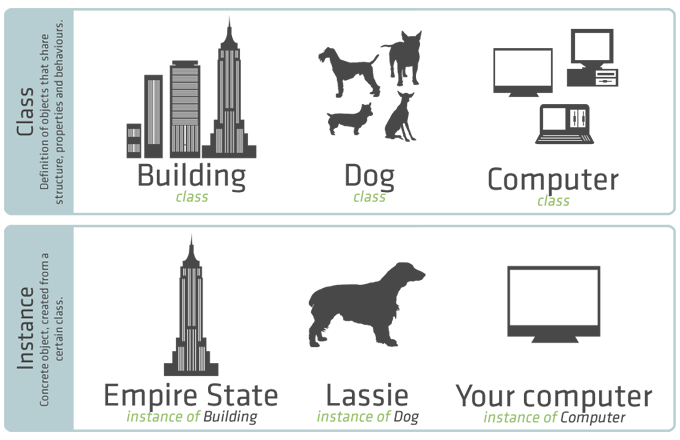
\includegraphics[width=0.8\linewidth]{classes_instances.png}
\caption{Graphical representation of a class instance.}
\end{figure}

To see how they can be defined let's try to code a class representing a person:

\begin{Verbatim}[commandchars=\\\{\}]
\PY{k+kn}{from} \PY{n+nn}{datetime} \PY{k}{import} \PY{n}{date}        
\PY{c+c1}{\PYZsh{} this is the class definition}
\PY{c+c1}{\PYZsh{} usually classes use camel naming convention}
\PY{k}{class} \PY{n+nc}{Person}\PY{p}{:}
   
   \PY{c+c1}{\PYZsh{} the special method \PYZus{}\PYZus{}init\PYZus{}\PYZus{} allows to instanciate a class}
   \PY{c+c1}{\PYZsh{} with an initial dataset (in this example a name and a birthday)}
   \PY{k}{def} \PY{n+nf}{\PYZus{}\PYZus{}init\PYZus{}\PYZus{}}\PY{p}{(}\PY{n+nb+bp}{self}\PY{p}{,} \PY{n}{name}\PY{p}{,} \PY{n}{date\PYZus{}of\PYZus{}birth}\PY{p}{)}\PY{p}{:}
       \PY{c+c1}{\PYZsh{} attribute of the class Person}
       \PY{c+c1}{\PYZsh{} name and self.name are different variable !!!}
       \PY{c+c1}{\PYZsh{} name will be destroyed once \PYZus{}\PYZus{}init\PYZus{}\PYZus{} is processed}
       \PY{c+c1}{\PYZsh{} self.name lives with every particualar instance of Person}
       \PY{n+nb+bp}{self}\PY{o}{.}\PY{n}{name} \PY{o}{=} \PY{n}{name} 
       \PY{c+c1}{\PYZsh{} attribute of the class Person}
       \PY{n+nb+bp}{self}\PY{o}{.}\PY{n}{date\PYZus{}of\PYZus{}birth} \PY{o}{=} \PY{n}{date\PYZus{}of\PYZus{}birth} 
       
   \PY{c+c1}{\PYZsh{} this normal method computes the current age of the}
   \PY{c+c1}{\PYZsh{} \PYZdq{}instanciated\PYZdq{} person}
   \PY{k}{def} \PY{n+nf}{age}\PY{p}{(}\PY{n+nb+bp}{self}\PY{p}{)}\PY{p}{:}
       \PY{n}{today} \PY{o}{=} \PY{n}{date}\PY{o}{.}\PY{n}{today}\PY{p}{(}\PY{p}{)}
       \PY{n}{age} \PY{o}{=} \PY{n}{today}\PY{o}{.}\PY{n}{year} \PY{o}{\PYZhy{}} \PY{n+nb+bp}{self}\PY{o}{.}\PY{n}{date\PYZus{}of\PYZus{}birth}\PY{o}{.}\PY{n}{year}
       \PY{k}{if} \PY{n}{today}\PY{o}{.}\PY{n}{month} \PY{o}{\PYZlt{}} \PY{n+nb+bp}{self}\PY{o}{.}\PY{n}{date\PYZus{}of\PYZus{}birth}\PY{o}{.}\PY{n}{month} \PY{o+ow}{or} \PYZbs{}
           \PY{n}{today}\PY{o}{.}\PY{n}{day} \PY{o}{\PYZlt{}} \PY{n+nb+bp}{self}\PY{o}{.}\PY{n}{date\PYZus{}of\PYZus{}birth}\PY{o}{.}\PY{n}{day}\PY{p}{:}
           \PY{n}{age} \PY{o}{\PYZhy{}}\PY{o}{=} \PY{l+m+mi}{1}
       \PY{k}{return} \PY{n}{age}
\end{Verbatim}

First of all the necessary modules are imported, in this case the \texttt{datetime} module is used to managed the person age.
Then the \texttt{class} keyword followed by the class name is used to start the actual class definition. In a sepate block of code all the class methods are defined like normal functions, you can see \texttt{\_\_init\_\_} and \texttt{age} here. These are examples of two kind of methods:

\begin{itemize}
\tightlist
\item normal methods which use or modify the instance attributes;
\item special methods, which define the class behaviour: you can spot these because they start and end with two underscores (\_\_).
\end{itemize}

\texttt{\_\_init\_\_} is the simplest example of special methods, it is called every time a class is instanciated (e.g. when you write me = Person(\ldots{})) and initializes the attributes of the class, in our example assign values to the \texttt{name} and \texttt{date\_of\_birth} attributes.

Another peculiarity of class methods with respect to standard functions is that they always take as first argument \texttt{self}. The \texttt{self} keyword is very important since allows a method to use the class attributes. Basically if you need to use the \texttt{name} attribute you have to type \texttt{self.name}. 

There are lots of other things you can do with classes, but this is enough for now. So let's try to play a bit with our example:

\begin{Verbatim}[commandchars=\\\{\}]
\PY{c+c1}{\PYZsh{} here we instanciate (create an instance of) the class }
\PY{c+c1}{\PYZsh{} in other words we \PYZdq{}specialize\PYZdq{} a generic Person with some data}
        
\PY{n}{me} \PY{o}{=} \PY{n}{Person}\PY{p}{(}\PY{l+s+s2}{\PYZdq{}}\PY{l+s+s2}{Matteo}\PY{l+s+s2}{\PYZdq{}}\PY{p}{,} \PY{n}{date}\PY{p}{(}\PY{l+m+mi}{1974}\PY{p}{,} \PY{l+m+mi}{10}\PY{p}{,} \PY{l+m+mi}{20}\PY{p}{)}\PY{p}{)}
  \PY{n+nb}{print} \PY{p}{(}\PY{n+nb}{type}\PY{p}{(}\PY{n}{me}\PY{p}{)}\PY{p}{)}
\end{Verbatim}

Once we have create an instance of a class its methods and attributes can be accessed again with the dot notazion: \texttt{instance\_name.method\_name}.

\begin{Verbatim}[commandchars=\\\{\}]
\PY{c+c1}{\PYZsh{} to access class attributes you have to use .}
\PY{n}{me}\PY{o}{.}\PY{n}{name}
\end{Verbatim}

\begin{Verbatim}[commandchars=\\\{\}]
\PY{n}{me}\PY{o}{.}\PY{n}{date\PYZus{}of\PYZus{}birth}
\end{Verbatim}

\begin{Verbatim}[commandchars=\\\{\}]
\PY{c+c1}{\PYZsh{} to call a class method you have to use . }
\PY{c+c1}{\PYZsh{} passing the parameters if needed}
\PY{n}{me}\PY{o}{.}\PY{n}{age}\PY{p}{(}\PY{p}{)}
\end{Verbatim}

Let's try to add more functionality to our class, adding a method that simply prints the age of the person in nice format. So complete the \texttt{Person} class with the following code:

\begin{Verbatim}[commandchars=\\\{\}]
    \PY{c+c1}{\PYZsh{} methods in a class are just functions which can work}
    \PY{c+c1}{\PYZsh{} with the class attributes}
    \PY{c+c1}{\PYZsh{} Remember I told you functions can have no return ?}
    \PY{k}{def} \PY{n+nf}{print\PYZus{}age}\PY{p}{(}\PY{n+nb+bp}{self}\PY{p}{)}\PY{p}{:}
        \PY{n+nb}{print} \PY{p}{(}\PY{l+s+s2}{\PYZdq{}}\PY{l+s+si}{\PYZob{}\PYZcb{}}\PY{l+s+s2}{ is }\PY{l+s+si}{\PYZob{}\PYZcb{}}\PY{l+s+s2}{ years old right now}\PY{l+s+s2}{\PYZdq{}}\PYZbs{}
               \PY{o}{.}\PY{n}{format}\PY{p}{(}\PY{n+nb+bp}{self}\PY{o}{.}\PY{n}{name}\PY{p}{,} \PY{n+nb+bp}{self}\PY{o}{.}\PY{n}{age}\PY{p}{(}\PY{p}{)}\PY{p}{)}\PY{p}{)}
\end{Verbatim}

Then try to test the new method by instanciating a new ``person'' and print her age.

\begin{Verbatim}[commandchars=\\\{\}]
\PY{n}{her} \PY{o}{=} \PY{n}{Person}\PY{p}{(}\PY{l+s+s2}{\PYZdq{}}\PY{l+s+s2}{Francesca}\PY{l+s+s2}{\PYZdq{}}\PY{p}{,} \PY{n}{date}\PY{p}{(}\PY{l+m+mi}{1986}\PY{p}{,} \PY{l+m+mi}{1}\PY{p}{,} \PY{l+m+mi}{27}\PY{p}{)}\PY{p}{)}
\PY{n}{print} \PY{p}{(}\PY{n}{her}\PY{o}{.}\PY{n}{print\PYZus{}age}\PY{p}{(}\PY{p}{)}\PY{p}{)}

34
\end{Verbatim}


